Chương này trình bày những kiến thức cơ sở để triển khai luận văn này, gồm:
\begin{itemize}
\item Kiểm thử phần mềm
\item Sinh ngẫu nhiên dữ liệu thử
\item Kỹ thuật Dynamic Symbolic Execution.
\end{itemize}

\section{Kiểm thử phần mềm}
	\subsection{Các khái niệm cơ bản trong kiểm thử phần mềm}
	\subsubsection{Khái niệm về kiểm thử phần mềm}
	\begin{itemize}
		\item Kiểm thử phần mềm là quá trình khảo sát một hệ thống hay thành phần dưới những điều kiện xác định, quan sát và ghi lại các kết quả, và đánh giá một khía cạnh nào đó của hệ thống hay thành phần đó \cite{radatz1990ieee}.
		
		\item Kiểm thử phần mềm là hoạt động khảo sát thực tiễn sản phẩm hay dịch vụ phần mềm trong đúng môi trường chúng dự định sẽ được triển khai nhằm cung cấp cho người có lợi ích liên quan những thông tin về chất lượng của sản phẩm hay dịch vụ phần mềm ấy. Mục đích của kiểm thử phần mềm là tìm ra các lỗi hay khiếm khuyết phần mềm nhằm đảm bảo hiệu quả hoạt động tối ưu của phần mềm trong nhiều ngành khác nhau \cite{wikipedia}.
		
		\item Chúng ta có thể định nghĩa như sau: Kiểm thử phần mềm là một tiến trình hay một tập hợp các tiến trình được thiết kế để đảm bảo phần mềm hoạt động đúng theo cái mà chúng đã được thiết kế, và không thực hiện bất cứ thứ gì không mong muốn. Đây là một bước quan trọng trong quá trình phát triển hệ thống, giúp cho người xây dựng hệ thống và khách hàng thấy được hệ thống mới đã đáp ứng yêu cầu đặt ra hay chưa.
	\end{itemize}

	\subsubsection{Mục đích của kiểm thử phần mềm}
	\begin{itemize}
		\item Tìm ra nhiều lỗi bằng việc đưa ra các dòng thời gian.
		\item Chứng minh được sản phẩm hoàn thành có những chức năng hay ứng dụng giống với bản đặc tả yêu cầu.
		\item Tạo ra các test case có chất lượng cao, thực thi hiệu quả…
		\item Một số lỗi cơ bản trong kiểm thử phần mềm như: lỗi ngay từ khi phân tích yêu cầu, lỗi từ bản đặc tả hệ thống, lỗi trong code, lỗi hệ thống và nguồn tài nguyên hệ thống, lỗi trong vấn đề phần mềm, phần cứng…		
	\end{itemize}

	\subsubsection{Các phương pháp kiểm thử}
	\begin{itemize}
		\item Kiểm thử tĩnh( Static testing): Là phương pháp thử phần mềm đòi hỏi phải duyệt lại các yêu cầu và các đặc tả bằng tay, thông qua việc sử dụng giấy, bút để kiểm tra logic, lần từng chi tiết mà không cần chạy chương trình. Kiểu kiểm thử này thường được sử dụng bởi chuyên viên thiết kế người mà viết mã lệnh một mình.
		
		Kiểm thử tĩnh cũng có thể được tự động hóa. Nó sẽ thực hiện kiểm tra toàn bộ bao gồm các chương trình được phân tích bởi một trình thông dịch hoặc biên dịch mà xác nhận tính hợp lệ về cú pháp của chương trình.
		
		\item Kiểm thử động (Dynamic testing): Là phương pháp kiểm thử thông qua việc dùng máy chạy chương trình để điều tra trạng thái tác động của chương trình. Đó là kiểm thử dựa trê các ca kiểm thử xác định bằng sự thực hiện của đối tượng kiểm thử hay chạy các chương trình. Kiểm thử động là kiểm tra cách thức hoạt động của mã lệnh, tức là kiểm tra sự phản ứng vật lý từ hệ thống tới các biến luôn thay đổi theo thời gian. Trong kiểm thử động, phần mềm phải thực sự được biên dịch và chạy. Kiểm thử động thực sự bao gồm làm việc với phần mềm, nhập các giá trị đầu vào và kiểm tra xem liệu đầu ra có như mong muốn hay không.
		
		Các phương pháp kiểm thử động gồm có kiểm thử mức đơn vị – Unit Tests, kiểm thử tích hợp – Intergration Tests, kiểm thử hệ thống – System Tests, và kiểm thử chấp nhận sản phẩm – Acceptance Tests.		
	\end{itemize}

	\subsubsection{Các chiến lược kiểm thử}
	Trong chiến lược kiểm thử, chúng ta có ba chiến lược kiểm thử hay dùng nhất là: kiểm thử hộp đen, kiểm thử hộp trắng, và kiểm thử hộp xám.
	\begin{itemize}
		\item Kiểm thử hộp đen – Black box
		Một trong những chiến lược kiểm thử quan trọng là kiểm thử hộp đen, hướng dữ liệu, hay hướng vào ra. Kiểm thử hộp đen xem chương trình như là một “hộp đen” và hoàn toàn không quan tâm về cách cư xử và cấu trúc bên trong của chương trình. Thay vào đó là tập trung vào tìm các trường hợp mà chương trình không thực hiện theo các đặc tả của nó.
		
		Kiểm thử hộp đen không có mối liên quan nào tới mã lệnh và kiểm thử viên chỉ rất đơn giản tam niệm là: một mã lệnh phải có lỗi. Sử dụng nguyên tắc “Hãy đòi hỏi và bạn sẽ được nhận”, những kiểm thử viên hộp đen tìm ra lỗi mà những lập trình viên không tìm ra. Nhưng, người ta nói kiểm thử hộp đen “giống như là đi trong bóng tối mà không có đèn vậy”, bởi vì kiểm thử viên không biết các phần mềm được kiểm tra thực sự được xây dựng như thế nào. Đó là lý do mà có nhiều trường hợp mà một kiểm thử viên hộp đen viết rất nhiều ca kiểm thử để kiểm tra một thứ gì đó mà đáng lẽ có thể chỉ cần kiểm tra bằng 1 ca kiểm thử duy nhất, và hoặc một số phần của chương trình không được kiểm tra chút nào.
		
		Do vậy, kiểm thử hộp đen có ưu điểm của “một sự đánh giá khách quan”, mặt khác nó lại có nhược điểm của “thăm dò mù”.
		
		\item Kiểm thử hộp trắng – White box.
		Là một chiến lược kiểm thử khác, trái ngược hoàn toàn với kiểm thử hộp đen, kiểm thử hộp trắng hay kiểm thử hướng logic cho phép bạn khảo sát cấu trúc bên trong của chương trình. Chiến lược này xuất phát từ dữ liệu kiểm thử bằng sự kiểm thử tính logic của chương trình. Kiểm thử viên sẽ truy cập vào cấu trúc dữ liệu và giải thuật bên trong chương trình (và cả mã lệnh thực hiện chúng).
		
		Phương pháp kiểm thử hộp trắng cũng có thể được sử dụng để đánh giá sự hoàn thành của một bộ kiểm thử mà được tạo cùng với các phương pháp kiểm thử hộp đen. Điều này cho phép các nhóm phần mềm khảo sát các phần của 1 hệ thống ít khi được kiểm tra và đảm bảo rằng những điểm chức năng quan trọng nhất đã được kiểm tra.
		
		\item Kiểm thử hộp xám – Gray box testing
		Kiểm thử hộp xám đòi hỏi phải có sự truy cập tới cấu trúc dữ liệu và giải thuật bên trong cho những mục đích thiết kế các ca kiểm thử, nhưng là kiểm thử ở mức người sử dụng hay mức hộp đen. Việc thao tác tới dữ liệu đầu vào và định dạng dữ liệu đầu ra là không rõ ràng, giống như một chiếc “hộp xám”, bởi vì đầu vào và đầu ra rõ ràng là ở bên ngoài “hộp đen” mà chúng ta vẫn gọi về hệ thống được kiểm tra. Sự khác biệt này đặc biệt quan trọng khi quản lý kiểm thử tích hợp – Intergartion testing giữa 2 modun mã lệnh được viết bởi hai chuyên viên thiết kế khác nhau, trong đó chỉ giao diện là được đưa ra để kiểm thử. Kiểm thử hộp xám có thể cũng bao gồm cả thiết kế đối chiếu để quyết định, ví dụ, giá trị biên hay thông báo lỗi.				
		
	\end{itemize}

	\subsubsection{Các cấp độ kiểm thử trong kiểm thử phần mềm}
	Kiểm thử phần mềm gồm có các cấp độ: 
	\begin{itemize}
		\item Kiểm thử đơn vị
		\item Kiểm thử tích hợp
		\item Kiểm thử hệ thống
		\item Kiểm thử chấp nhận sản phẩm
	\end{itemize}
	
	\begin{center}
		\begin{figure}[htp]
			\begin{center}
				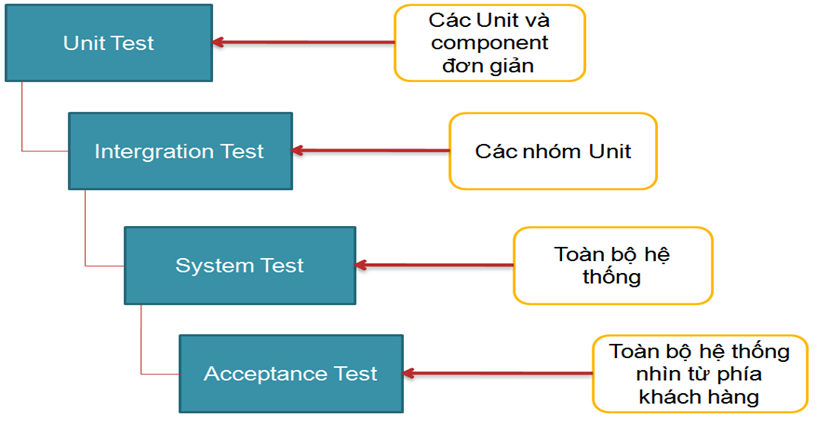
\includegraphics[scale=.3]{giai-doan-kiem-thu-1.png}
			\end{center}
			\caption{Sơ đồ các cấp độ kiểm thử}
			\label{refhinh1}
		\end{figure}
	\end{center}
	

	

	\subsection{Đảm bảo chất lượng phần mềm}
	\textbf{Định nghĩa theo Daniel Galin \cite{galin2004software}:} Đảm bảo chất lượng phần mềm là một tập hợp các hành động được lên kế hoạch một cách hệ thống để cung cấp đầy đủ niềm tin rằng quá trình phát triển phần mềm phù hợp để thành lập các yêu cầu chức năng kỹ thuật cũng như các yêu cầu quản lý theo lịch trình và hoạt động trong giới hạn.


\section{Sinh ngẫu nhiên dữ liệu thử}

	%Phần này trình bày cơ bản về sinh dữ liệu thử ngẫu nhiên, những ưu và nhược điểm cùng những cải tiến để nâng cao hiệu quả.

	Trong kiểm thử phần mềm, các ca kiểm thử thường được tạo ra thủ công do đó sẽ gây ra tốn kém chi phí và mất nhiều thời gian để hoàn thành phần mềm. Hiện nay, đã có nhiều phương pháp hỗ trợ việc sinh tự động các ca kiểm thử một cách có hệ thống, một phương pháp đơn giản nhất đó là kiểm thử ngẫu nhiên (random testing) \cite{zhu1997software}. Giả sử, với một hạm nhận giá trị đầu vào có kiểu string thì chỉ cần sinh ngẫu nhiên một luồng các bits để thể hiện cho một chuỗi. Kiểm thử ngẫu nhiên có ưu điểm là dễ dàng sinh các đầu vào ngẫu nhiên và hệ thống kiểm thử ngẫu nhiên không yêu cầu bộ nhớ lúc thực thi. Nhưng hạn chế của nó là kiểm tra cùng 1 hành vi thực thi của chương tình nhiều lần với những đầu vào khác nhau và chỉ có thể kiểm tra được một số trường hợp thực thi của chương trình. Ngoài ra, kiểm thử ngẫu nhiên khó xác định khi nào việc kiểm thử nên dừng lại và không biết không gian trạng thái đã được thám hiểm hết hay chưa.
	
	Một giải pháp giúp khắc phục những hạn chế của kiểm thử ngẫu nhiên đó là việc thực thi tượng trưng (Symbolic execution) \cite{king1976symbolic}. Việc thực thi tượng trưng là việc xây dựng các ràng buộc dựa vào các giá trị tượng trưng và giải quyết các giá trị tương trưng đó để sinh ra giá trị đầu vào của chương trình mà có thể thực thi chương trình theo các đường đi thực thi khác nhau. Ý tưởng chính của thực thi tượng trưng đó là thực thi một chương trình với những giá trị tượng trưng. Có hai cách tiếp cận với thực thi tượng trưng đó là cách tiếp cận dựa trên phân tích tĩnh và phân tích động chương trình


\section{Kỹ thuật Dynamic symbolic execution}

	Kỹ thuật Dynamic Symbolic Execution (DSE) \cite{xie2009fitness} là một kỹ thuật thực thi tượng trưng dựa trên phân tích chương trình động. DSE chính là sự kết hợp giữa thực thi cụ thể và thực thi tượng trưng. Trong thực thi tượng trưng động, chương trình được thực thi nhiều lần với những giá trị khác nhau của tham số đầu vào.

	Bắt đầu bằng việc chọn những tham số tùy ý cho các tham số đầu vào và thực thi chương trình với những giá trị cụ thể đó. Với những giá trị cụ thể này thì chương trình sẽ được thực thi theo một đường đi xác định. Thực thi chương trình với các giá trị cụ thể của tham số đầu vào và thu gom các ràng buộc trong quá trình thực thi theo đường đi mà sự thực thi cụ thể này đi theo, đồng thời suy ra những ràng buộc mới từ những ràng buộc đã thu gom được.

	Tại các câu lệnh rẽ nhánh, biểu thức điều kiện rẽ nhánh sẽ được đánh giá phụ thuộc vào các giá trị cụ thể của tham số đầu vào. Nếu biểu thức rẽ nhánh nhận giá trị là True thì biểu thức của điều kiện rẽ nhánh sẽ được thu gom vào ràng buộc của PC và được ghi nhớ, đồng thời phủ định của điều kiện rẽ nhánh sẽ được sinh ra và sẽ được thêm vào một PC tương ứng với nhánh còn lại mà thực thi cụ thể đó không đi theo. Một bộ xử lý ràng buộc (Constraint Solver) sẽ được sử dụng để giải các ràng buộc mới sinh ra này để sinh ra các giá trị cụ thể của tham số đầu vào. Ngược lại nếu biểu thức rẽ nhánh nhận giá trị là False thì biểu thức điều kiện rẽ nhánh sẽ được thu gom vào ràng buộc của PC tương ứng với nhánh đi mà sự thực thi hiện thời đang đi theo và được ghi nhớ. Đồng thời điều kiện rẽ nhánh sẽ được sinh ra và thêm vào PC tương ứng với nhánh đi còn lại mà sự thực thi hiện thời không đi theo. Các giá trị mới được sinh ra của các tham số đầu vào sẽ tiếp tục được thực thi và quá trình này sẽ được lập lại cho tới khi chương trình thực thi theo tất cả các đường đi.

	Do các chương trình được thực thi với những giá trị cụ thể nên có thể thấy rằng, tất cả các đường đi phân tích được trong quá trình thực thi tượng trưng động đều là các đường đi khả thi.

	\textbf{Thuật toán Dynamic symbolic execution}
	\begin{itemize}
		\item S: Tập hợp các lệnh của chương trình P
		\item s: Tập con của S (s $\subseteq $ S)
		\item I: Tập hợp các đầu vào của P
		\item P(i): Thực thi chương trình đầu vào i $\in $ I, sao cho s được thực thi
		\item J: Tập hợp các đầu vào của P được thực thi (J = {i|P(i)})
		\item C(i): Ràng buộc thu gom từ việc thực thi P(i), hay còn gọi là điều kiện đường đi 
		\item C'(i): Điều kiện đường đi suy ra từ C(i)
		
		Bước 0: J:= {} (tập rỗng)
		
		Bước 1: Chọn đầu vào i không thuộc j (dừng lại nếu không có i nào được tìm ra)
		
		Bước 2: Output i
		
		Bước 3: Thực thi P(i); ghi nhớ đường đi C(i), suy ra C'(i)
		
		Bước 4: Đặt J := J $\cup $ i
		
		Bước 5: Quay lại bước 1
		
	\end{itemize}
	
	
	Hiện nay, đã có những nghiên cứu về cách giải quyết các ràng buộc như Z3 \cite{de2008z3}, và nhiều công cụ sử dụng kỹ thuật DSE để giải quyết các ràng buộc và tạo ra các giá trị đầu vào có độ phủ cao như như Pex \cite{tillmann2008pex} và SAGE \cite{godefroid2008automated}... hỗ trợ trên nhiều ngôn ngữ và nền tảng khác nhau.
	
	Và một số công cụ khác:
	\begin{center}
		\begin{tabular}  {|c|c|c|} 
			\hline 
			\textbf{Tên Công cụ} & \textbf{Ngôn ngữ} & \textbf{Url} \\ 
			\hline 
			KLEE & LLVM & klee.github.io/ \\ 
			\hline 
			JPF	 & Java	& babelfish.arc.nasa.gov/trac/jpf \\
			\hline 
			jCUTE &	Java &	github.com/osl/jcute \\
			\hline 
			janala2	 & Java &	github.com/ksen007/janala2 \\
			\hline 
			JBSE	& Java	 & github.com/pietrobraione/jbse \\
			\hline 
			KeY &	Java &	www.key-project.org/ \\	
			\hline 
			Mayhem & 	Binary &	forallsecure.com/mayhem.html \\
			\hline 
			Otter &	C	& bitbucket.org/khooyp/otter/overview \\
			\hline 
			Rubyx & 	Ruby &	www.cs.umd.edu/~avik/papers/ssarorwa.pdf \\
			\hline 
			Pex	& .NET Framework	 & research.microsoft.com/en-us/projects/pex/ \\
			\hline 
			Jalangi2 &	JavaScript &	github.com/Samsung/jalangi2 \\
			\hline 
			Kite &	LLVM &	www.cs.ubc.ca/labs/isd/Projects/Kite/ \\
			\hline 
			pysymemu &	x86-64 / Native	 &github.com/feliam/pysymemu/ \\
			\hline 
			Triton	& x86 and x86-64 &	triton.quarkslab.com \\	
			\hline 
			BE-PUM &	x86	 & https://github.com/NMHai/BE-PUM	 \\	
			\hline
			
		\end{tabular} 

	\end{center}
	
\section*{Tổng kết chương}
%Tổng kết chương viết ở đây.
Chương này, trình bày khái quát và sơ lượt những kiến thức như: Kỹ thuật kiểm thử phần mềm; các kỹ thuật sinh dữ liệu thử; kỹ thuật Dynamic symbolic execution. Những kiến thức này, giúp chúng ta có cái nhìn tổng quan về cách thức kiểm thử phần mềm, giải quyết các ràng buộc trong chường trình tìm ra các giá trị thử nghiệm có độ phủ cao.


